\documentclass[11pt]{article}

\usepackage[margin=1.1in]{geometry}
\usepackage{amsmath,amssymb,amsthm}
\usepackage{dsfont}
% shim: dual_coefficient_mappings.tex uses \mathbbm; the bbm fonts lack
% Type1 versions, so map onto doublestroke
\newcommand{\mathbbm}[1]{\mathds{#1}}
\usepackage{graphicx}
\usepackage{booktabs}
\usepackage{algorithm}
\usepackage{algorithmic}
\usepackage[round]{natbib}
\usepackage[colorlinks=true,linkcolor=blue,citecolor=blue,urlcolor=blue]{hyperref}

\newtheorem{theorem}{Theorem}
\newtheorem{lemma}{Lemma}
\newtheorem{corollary}{Corollary}
\newtheorem{proposition}{Proposition}
\theoremstyle{remark}
\newtheorem{remark}{Remark}
\newtheorem{example}{Example}

\title{Bipartite Ranking with the Pairwise Hinge is Balanced
Classification over a Transportation Polytope}
\author{Jesse Glass}
\date{Draft of \today}

\begin{document}
\maketitle

\begin{abstract}
We show that the dual of the pairwise-hinge bipartite ranking SVM (RankSVM)
is \emph{exactly} the dual of a balanced cost-sensitive classification SVM,
restricted to a capacitated transportation polytope. Under a margin-2
convention the two dual objectives coincide -- not merely up to constants --
and the classification intercept constraint arises automatically. We
characterize the restricted domain exactly: it is the convex hull of
per-example \emph{misordering-count} vectors, described by Gale-type
inequalities, with membership decidable by a single maximum-flow computation
that also returns a dual witness. Consequences: (i) the balanced solution
lower-bounds the RankSVM dual optimum, and any transportation-feasible point
upper-bounds it, giving a computable optimality certificate; (ii) every
Frank--Wolfe step on the pairwise dual is a sample-weighted classification
problem whose weights count misordered opposite-class examples, and balanced
classification is precisely the first Frank--Wolfe step; (iii) at the
gradient level the equivalence holds for \emph{any} differentiable scorer:
the parameter gradient of a decomposable pairwise loss equals the gradient of
a count-weighted univariate loss, computable in $O(N\log N)$ without forming
pairs. This geometry unifies a family of known efficiency results and
reweighting heuristics -- structural-SVM cutting planes, sorted-gradient
RankSVM solvers, LambdaMART's per-document lambdas, hard-example mining --
as views of one object. Experiments confirm the theory's predictions,
including the negative ones: count-reweighted classifiers match RankSVM and
pairwise-loss networks everywhere at a fraction of the cost, while offering
only situational gains over static balanced weighting, exactly as
AUC-consistency theory implies.
\end{abstract}

\section{Introduction}
\label{sec:intro}

Bipartite ranking asks for a scoring function that places positive examples
above negative ones; its canonical empirical objective is the area under the
ROC curve (AUC), and its canonical convex surrogate is the pairwise hinge
over all positive--negative pairs \citep{herbrich2000,joachims2002}. Taken
literally, the pairwise objective couples $n^+ n^-$ terms, and a substantial
literature exists on evaluating or optimizing it without enumerating pairs
\citep{joachims2005,chapelle2010,airola2011,ying2016}. A parallel statistical
literature shows that pairs are unnecessary in a deeper sense: minimizing a
class-balanced \emph{univariate} loss is AUC-consistent, with explicit
surrogate regret bounds \citep{kotlowski2011,agarwal2014}.

This paper gives the exact finite-sample geometry underlying both
observations. Our main results concern the Lagrangian duals of the two
problems. Let the pairwise SVM be taken with margin $2$ (a rescaling of the
standard formulation; Remark~\ref{rem:margin2}) and let the balanced
classification SVM weight each example by the empirical frequency of the
\emph{opposite} class. Then, under the natural row/column-sum map from pair
multipliers to example multipliers:
\begin{enumerate}
\item \textbf{Equivalence (Theorem~\ref{thm:equivalence}).} The pairwise dual
objective \emph{equals} the balanced classification dual objective -- same
quadratic form, same linear term -- and the intercept constraint of the
classification dual holds automatically. The pairwise dual is the balanced
dual restricted to a subdomain $\mathcal{T}$.
\item \textbf{Geometry (Theorem~\ref{thm:image}).} $\mathcal{T}$ is a
capacitated transportation polytope: the convex hull of scaled
\emph{misordering-count} vectors, cut out by Gale-type inequalities
\citep{gale1957}, with membership decidable by one max-flow computation on a
network with $n^+ + n^- + 2$ nodes (Corollary~\ref{cor:membership}). It is
strictly smaller than the balanced dual's box-plus-hyperplane domain.
\item \textbf{Certificate (Corollary~\ref{cor:sandwich}).} The balanced
optimum lower-bounds the pairwise optimum; any point of $\mathcal{T}$
upper-bounds it. The gap is computable and vanishes exactly when the
balanced solution is transportation-feasible.
\item \textbf{Beyond linear models (Proposition~\ref{prop:gradient}).} For
any differentiable scorer, the parameter gradient of a decomposable pairwise
loss equals the gradient of a per-example loss weighted by (soft) violation
counts, frozen at the current scores. Count-reweighted training \emph{is}
pairwise training at the gradient level, at $O(N \log N)$ per evaluation for
the hinge.
\end{enumerate}
The picture that emerges is summarized by
Corollary~\ref{cor:fw_bridge}: running Frank--Wolfe
\citep{frank1956,jaggi2013} on the pairwise dual is running Frank--Wolfe on
$\mathcal{T}$, each linear-minimization step is a weighted classification
problem whose weights are misordering counts, and \emph{balanced
classification is exactly the first step}. This explains, in one frame, why
balanced univariate training is so hard to beat for AUC
\citep{kotlowski2011}, why structural-SVM cutting planes for ROC area reduce
to sorting \citep{joachims2005}, why primal RankSVM gradients collapse to
per-example counts \citep{chapelle2010}, why gradient-boosted ranking works
from per-document ``lambdas'' \citep{burges2010}, and why hard-example
mining heuristics \citep{shrivastava2016,lin2017} succeed: each example's
principled ``hardness'' weight is the number of opposite-class examples that
outrank it.

We claim no new state-of-the-art method, and our experiments
(Section~\ref{sec:experiments}) are designed to test the theory's
predictions rather than to win benchmarks. They confirm: count-reweighted
classifiers reproduce RankSVM (linear) and pairwise-logistic training (MLPs)
within noise on every dataset tried, at $1.3$--$4.4\times$ lower cost per
epoch and better asymptotic complexity; iterated reweighting with
cross-fitted model selection behaves as a ``free option'' over balanced
weighting -- it selects the balanced solution when that is optimal and
harvests modest gains when headroom exists; and, as consistency theory
predicts, neither pairwise training nor its reweighted equivalent broadly
beats plain or balanced univariate baselines on generic tabular data. The
contribution is the geometry, the certificate, and the unification.

\section{Related Work}
\label{sec:related}

\paragraph{Efficient pairwise training.} That the pairwise hinge can be
optimized without materializing pairs is well established.
\citet{joachims2005} trains an ROC-area structural SVM whose cutting-plane
oracle runs in $O(N \log N)$ by sorting; \citet{joachims2006} shows the
error-rate structural SVM is equivalent to a classification SVM.
\citet{chapelle2010} solve primal RankSVM with Newton methods whose
objective and gradient are evaluated in $O(N \log N)$; \citet{airola2011}
achieve linearithmic training with order-statistic trees. In learning to
rank, LambdaRank/LambdaMART collapse pairwise gradients into per-document
weights \citep{burges2010}. For the square surrogate, \citet{ying2016}
remove pairs entirely via a min-max reformulation, the basis of large-scale
deep AUC maximization \citep{yuan2021,yang2022}. Our contribution relative
to this line is not efficiency but structure: these algorithms implicitly
traverse the transportation polytope $\mathcal{T}$; we name the object,
characterize it exactly, and equip it with a membership test and an
optimality certificate none of the above provide.

\paragraph{Statistical equivalences.} \citet{kotlowski2011} and
\citet{agarwal2014} show balanced univariate losses are AUC-consistent with
explicit regret transfer; \citet{ertekin2011} prove AdaBoost and RankBoost
are equivalent in a precise sense; \citet{clemencon2008} give the
$U$-statistics theory of pairwise ERM. These are asymptotic or
population-level statements; Theorem~\ref{thm:equivalence} is their exact
finite-sample, fixed-regularization counterpart at the level of dual
programs, and Corollary~\ref{cor:sandwich} quantifies the finite-sample gap
between balanced and pairwise solutions.

\paragraph{Frank--Wolfe for structured duals.} Block-coordinate Frank--Wolfe
for structural SVMs \citep{lacostejulien2013} popularized dual optimization
via linear-minimization oracles. Corollary~\ref{cor:fw_bridge} identifies
the pairwise-ranking LMO with a weighted classification problem, which makes
plug-in, dual-free implementations possible
(Section~\ref{sec:algorithms}).

\paragraph{Reweighting heuristics.} Online hard example mining
\citep{shrivastava2016}, focal loss \citep{lin2017}, and margin-based
weighted-classification losses in metric learning \citep{deng2019} weight
examples by difficulty. Proposition~\ref{prop:gradient} supplies the
principled special case: for bipartite objectives, the exact pairwise-loss
gradient is recovered by weighting each example with its count of violated
pairs.

% ---------------------------------------------------------------------------
% ============================================================================
% Dual Coefficient Mappings -- rewritten under the margin-2 convention.
% Drop-in replacement for the previous \section{Dual Coefficient Mappings}.
%
% Requires in the preamble: amsmath, amsthm, bbm, algorithm, algorithmic, and
% theorem environments named: theorem, lemma, corollary, proposition, remark,
% example. e.g.
%   \newtheorem{theorem}{Theorem}
%   \newtheorem{lemma}{Lemma}
%   \newtheorem{corollary}{Corollary}[theorem]
%   \newtheorem{proposition}{Proposition}
%   \theoremstyle{remark} \newtheorem{remark}{Remark} \newtheorem{example}{Example}
%
% Cross-reference notes: this version is self-contained; equations that
% previously lived elsewhere (eq:SVM_Lagrangian_Dual_Loss, eq:Wolfe_Dual_Loss,
% eq:Box_Constraints, eq:pair_hinge, eq:Struct_Pair_Margin) are restated here
% with new labels. Search for "TODO" to reconcile with the rest of the paper.
%
% Summary of changes from the previous draft:
%   1. Margin-2 pairwise hinge throughout: [2 - <w, x_i - x_j>]_+. This is the
%      convention under which the pairwise and balanced dual OBJECTIVES agree
%      exactly (previously the linear terms differed by a factor of 2). A
%      remark shows margin-2 with parameter C is standard RankSVM with C/2,
%      so nothing is lost.
%   2. The injectivity claim of old Theorem 3 is removed (it is false for
%      n+, n- >= 2: a "rectangle move" on rho preserves all row/column sums).
%      It is replaced by the observation that the dual objective factors
%      through lambda, which is what the algorithm actually needs.
%   3. The image of the pairwise dual domain is now characterized EXACTLY:
%      it is a capacitated transportation polytope, strictly smaller than
%      box-plus-bias-hyperplane, with (a) a convex-hull description matching
%      the Frank-Wolfe vertices and (b) a Gale-type inequality description
%      giving a polynomial-time membership test via max-flow.
%   4. Old Theorems 1-2 are demoted to background lemmas (the error-rate
%      structural SVM / classification SVM equivalence is essentially known;
%      cite Joachims 2005, 2006 and Lacoste-Julien et al. 2013). Their proofs
%      are cleaned: the layer-cake construction is stated precisely and the
%      non-injectivity argument is now a counterexample, not a "contrapositive".
%   5. The bias-constraint corollary is promoted into the main equivalence
%      theorem: the pairwise dual lands in the WITH-intercept balanced dual
%      feasible set automatically.
%   6. New sandwich/certificate corollary: the balanced solution lower-bounds
%      the pairwise dual optimum and any transportation-feasible point upper-
%      bounds it, which is the foundation of the successive-tightening
%      algorithm in the next section.
% ============================================================================

\section{Dual Coefficient Mappings}
\label{sec:dual_maps}

This section establishes the precise relationship between the pairwise
(bipartite-ranking) SVM and the balanced cost-sensitive classification SVM at
the level of their dual programs. The main results are: (i) under the natural
row/column-sum map, the pairwise dual \emph{objective} coincides exactly with
the balanced classification dual objective (Theorem~\ref{thm:equivalence});
(ii) the pairwise dual feasible set maps onto a \emph{capacitated
transportation polytope} strictly contained in the balanced dual feasible set,
with the intercept constraint of the classification SVM arising automatically
(Theorems~\ref{thm:equivalence} and~\ref{thm:image}); and (iii) membership in
this polytope is testable in polynomial time
(Corollary~\ref{cor:membership}). Consequently, bipartite ranking with the
pairwise hinge \emph{is} balanced cost-sensitive classification with
additional transportation constraints on the dual variables, and each
Frank--Wolfe vertex of the pairwise dual corresponds to a sample-weighted
classification problem whose weights count misordered opposite-class examples
(Corollary~\ref{cor:fw_bridge}). These results license the dual-variable-free
algorithms of the next section: we may optimize the pairwise dual entirely in
the space of univariate Lagrangian coefficients, successively tightening the
balanced domain toward the transportation polytope, and stopping early
whenever leaving the polytope improves the margin.

\subsection{Setup and conventions}
\label{sec:conventions}

Let $x_i$, $i = 1, \dots, n^+$ denote the positive examples and $x_j$,
$j = 1, \dots, n^-$ the negative examples, with $N = n^+ + n^-$,
$p = n^+/N$, $q = n^-/N$, and labels $t_k \in \{+1, -1\}$ indexed by
$k = 1, \dots, N$ (index $i$ ranges over positives, $j$ over negatives, $k$
over all examples, and $\pi = (i,j)$ over positive--negative pairs). Write
$z_\pi = x_i - x_j$ for the pair difference vectors,
$Q = t t^\top \odot X X^\top$ for the standard SVM Gram operator, and
\begin{equation}
\bar{C} \;=\; \frac{C}{N^2}
\label{eq:cbar}
\end{equation}
for the per-pair regularization weight.

\paragraph{Pairwise hinge, margin-2 convention.}
The pairwise (RankSVM) primal is taken with margin $2$:
\begin{equation}
\min_{w}\;\; \frac{1}{2}\|w\|^2
\;+\; \bar{C} \sum_{i=1}^{n^+} \sum_{j=1}^{n^-}
\bigl[\, 2 - \langle w, x_i - x_j \rangle \,\bigr]_+ .
\label{eq:pair_primal}
\end{equation}
Its Lagrangian dual, with one multiplier $\rho_\pi = \rho_{ij}$ per pair, is
\begin{equation}
\min_{\rho}\;\; \frac{1}{2} \rho^\top \widetilde{Q} \rho
\;-\; 2\,\mathbbm{1}^\top \rho
\qquad \text{s.t.} \quad 0 \le \rho_\pi \le \bar{C} \;\;\forall \pi,
\label{eq:pair_dual}
\end{equation}
where $\widetilde{Q}_{\pi\pi'} = \langle z_\pi, z_{\pi'} \rangle$ and
$w = \sum_\pi \rho_\pi z_\pi$ at optimality. There is no equality constraint
because the intercept cancels within each pair.

\begin{remark}[Margin~2 is standard RankSVM, rescaled]
\label{rem:margin2}
For any $w$, substituting $v = w/2$ in \eqref{eq:pair_primal} gives
\[
\frac{1}{2}\|w\|^2 + \bar{C}\sum_{\pi}\bigl[2 - \langle w, z_\pi\rangle\bigr]_+
= 4\left( \frac{1}{2}\|v\|^2
+ \frac{\bar{C}}{2}\sum_{\pi}\bigl[1 - \langle v, z_\pi\rangle\bigr]_+ \right).
\]
Hence the margin-2 problem with parameter $C$ has the same minimizer, up to
the scaling $w = 2v$, as the unit-margin RankSVM with parameter $C/2$. The
induced ranking function, the AUC, and the regularization path are unchanged;
only the parameterization of $C$ shifts. The margin-2 convention is the
natural one here because it is the margin produced by summing the two
univariate hinges of a pair:
$[1 - \langle w, x_i\rangle]_+ + [1 + \langle w, x_j\rangle]_+
\ge [2 - \langle w, x_i - x_j\rangle]_+$.
\end{remark}

\paragraph{Balanced classification.}
The balanced (class-weighted) binary SVM with intercept weights each positive
example by $\bar{C} n^-$ and each negative example by $\bar{C} n^+$:
\begin{equation}
\min_{w, b}\;\; \frac{1}{2}\|w\|^2
\;+\; \bar{C}\, n^- \sum_{i=1}^{n^+} \bigl[ 1 - (\langle w, x_i\rangle + b) \bigr]_+
\;+\; \bar{C}\, n^+ \sum_{j=1}^{n^-} \bigl[ 1 + (\langle w, x_j\rangle + b) \bigr]_+ .
\label{eq:bal_primal}
\end{equation}
(Equivalently, per-class weights $\tfrac{C}{N}q$ and $\tfrac{C}{N}p$: each
example is weighted by the empirical frequency of the \emph{opposite} class.)
Its dual, with one multiplier $\lambda_k$ per example, is
\begin{equation}
\min_{\lambda}\;\; D(\lambda) \;:=\; \frac{1}{2}\lambda^\top Q \lambda
\;-\; \mathbbm{1}^\top \lambda
\qquad \text{s.t.} \quad \lambda \in \mathcal{B},
\label{eq:bal_dual}
\end{equation}
\begin{equation}
\mathcal{B} \;=\; \Bigl\{ \lambda \in \mathbbm{R}^N_{\ge 0} \;:\;
\lambda_i \le \bar{C} n^- \;\forall i, \;\;
\lambda_j \le \bar{C} n^+ \;\forall j, \;\;
\textstyle\sum_k t_k \lambda_k = 0 \Bigr\},
\label{eq:bal_domain}
\end{equation}
with $w = \sum_k t_k \lambda_k x_k$ at optimality. The equality constraint in
\eqref{eq:bal_domain} is the usual consequence of the intercept $b$.

\subsection{Background: Frank--Wolfe and Lagrangian dual coefficients}
\label{sec:background}

The structural SVM and its (block-coordinate) Frank--Wolfe optimizers
% TODO: cite Joachims (2005, 2006); Lacoste-Julien, Jaggi, Schmidt, Pletscher (2013)
work with dual coefficients $\alpha$ indexed by \emph{joint labelings}
(vertices) rather than by examples. For a decomposable hinge, each vertex
$s \in \{0,1\}^N$ marks which examples are margin-violated, and the linear
operator $\mathcal{S}$, whose columns are the vertices, maps vertex
coefficients to example coefficients:
\begin{equation}
\lambda \;=\; \mathcal{S}\alpha,
\qquad
\alpha \in \Delta_C := \Bigl\{ \alpha \ge 0 : \textstyle\sum_s \alpha_s = C \Bigr\}.
\label{eq:wolfe_map}
\end{equation}
The two background lemmas below record that nothing is lost by tracking
$\lambda$ instead of $\alpha$; they are essentially the known equivalence
between the error-rate structural SVM and the classification SVM
% TODO: cite Joachims (2006), Theorem 1
and are stated in the form used later.

\begin{lemma}[Per-example blocks: bijection]
\label{lem:block_bijection}
In the block-separable formulation (one block per example, block mass $C_k$
equal to that example's primal weight), each block has two vertices --
violated and satisfied -- with coefficients $\alpha_{k1} + \alpha_{k0} = C_k$.
The map $\lambda_k = \alpha_{k1}$ is a bijection between the per-block
Frank--Wolfe domain and the Lagrangian box $\lambda_k \in [0, C_k]$, applied
independently across blocks.
\end{lemma}

\begin{proof}
Immediate: $\alpha_{k1} \in [0, C_k]$ determines $\alpha_{k0} = C_k -
\alpha_{k1}$ uniquely, and every $\lambda_k \in [0, C_k]$ is attained.
\end{proof}

\begin{lemma}[Holistic formulation: surjection onto the box]
\label{lem:holistic_surjection}
Let $\mathcal{S} \in \{0,1\}^{N \times 2^N}$ contain all binary vertices as
columns. The map $\alpha \mapsto \mathcal{S}\alpha$ sends $\Delta_C$
\emph{onto} $[0, C]^N$, using at most $N$ vertices with nested supports; it is
not injective for $N \ge 2$.
\end{lemma}

\begin{proof}
(\emph{Surjectivity: layer-cake construction.}) Fix $\lambda \in [0,C]^N$ and
let $0 < v_1 < v_2 < \cdots < v_r$ be its distinct positive values, with
$v_0 = 0$. Define nested vertices $s_m = \mathbbm{1}\{\lambda \ge v_m\}$ and
coefficients $\alpha_{s_m} = v_m - v_{m-1} > 0$ for $m = 1, \dots, r$. For each
coordinate $k$, $\sum_m \alpha_{s_m} (s_m)_k = \sum_{m : v_m \le \lambda_k}
(v_m - v_{m-1}) = \lambda_k$, so $\mathcal{S}\alpha = \lambda$. The
coefficients sum to $v_r = \max_k \lambda_k \le C$; assign the remainder
$C - v_r$ to the zero vertex $s_0 = \mathbf{0}$. This uses $r \le N$ nonzero
vertices plus the zero vertex, all with nested supports.

(\emph{Non-injectivity.}) For $N = 2$, the distinct points
$\alpha = \tfrac{C}{2}\bigl(e_{(1,1)} + e_{(0,0)}\bigr)$ and
$\widetilde{\alpha} = \tfrac{C}{2}\bigl(e_{(1,0)} + e_{(0,1)}\bigr)$
both map to $\lambda = (\tfrac{C}{2}, \tfrac{C}{2})$.
\end{proof}

For the pairwise loss, the vertices are subsets $s$ of positive--negative
pairs, and the corresponding column of $\mathcal{S}$ records, for each
example, \emph{how many} pairs in $s$ it participates in:
\begin{equation}
(\mathcal{S} e_s)_i \;=\; \#\{\, j : (i,j) \in s \,\}, \qquad
(\mathcal{S} e_s)_j \;=\; \#\{\, i : (i,j) \in s \,\}.
\label{eq:pair_counts}
\end{equation}
Under the margin-2 convention the structural loss of vertex $s$ is
$\Delta_s = 2|s|$ (each misordered pair contributes its margin), and since
each pair touches exactly two examples,
$\mathbbm{1}^\top \mathcal{S} e_s = 2|s| = \Delta_s$. Summing over vertices:
\begin{equation}
\Delta^\top \alpha \;=\; \mathbbm{1}^\top \mathcal{S} \alpha
\;=\; \mathbbm{1}^\top \lambda .
\label{eq:margin_identity}
\end{equation}
This is the pairwise analogue of the classification identity and is the
bookkeeping that makes Theorem~\ref{thm:equivalence} exact. (Under a
unit-margin convention the two sides differ by a factor of $2$; see
Remark~\ref{rem:margin2}.)

\subsection{The pairwise dual is a constrained balanced dual}
\label{sec:equivalence}

Define the row/column-sum map $\Phi$ from pair coefficients to example
coefficients:
\begin{equation}
\Phi(\rho) \;=\; \lambda, \qquad
\lambda_i = \sum_{j=1}^{n^-} \rho_{ij}, \qquad
\lambda_j = \sum_{i=1}^{n^+} \rho_{ij}.
\label{eq:phi_map}
\end{equation}

\begin{theorem}[Dual equivalence]
\label{thm:equivalence}
Let $\mathcal{R} = [0, \bar{C}]^{\,n^+ \times n^-}$ be the pairwise dual
feasible set \eqref{eq:pair_dual} and let $\lambda = \Phi(\rho)$. Then:
\begin{enumerate}
\item[(i)] \emph{(Weight vectors agree.)}
$\displaystyle \sum_\pi \rho_\pi z_\pi = \sum_k t_k \lambda_k x_k$.
\item[(ii)] \emph{(Objectives agree.)}
$\displaystyle \frac{1}{2}\rho^\top \widetilde{Q} \rho - 2\,\mathbbm{1}^\top\rho
= \frac{1}{2}\lambda^\top Q \lambda - \mathbbm{1}^\top\lambda = D(\lambda)$.
\item[(iii)] \emph{(Feasibility is preserved, intercept included.)}
$\Phi(\mathcal{R}) \subseteq \mathcal{B}$, where $\mathcal{B}$ is the
balanced feasible set \eqref{eq:bal_domain}. In particular the equality
constraint $\sum_k t_k \lambda_k = 0$ holds automatically for every
$\lambda \in \Phi(\mathcal{R})$.
\end{enumerate}
Consequently, with $\mathcal{T} := \Phi(\mathcal{R})$,
\begin{equation}
\min_{\rho \in \mathcal{R}}\;
\frac{1}{2}\rho^\top \widetilde{Q} \rho - 2\,\mathbbm{1}^\top\rho
\;\;=\;\;
\min_{\lambda \in \mathcal{T}}\; D(\lambda),
\label{eq:reduced_problem}
\end{equation}
i.e.\ the pairwise dual is exactly the balanced classification dual restricted
to the subdomain $\mathcal{T} \subseteq \mathcal{B}$.
\end{theorem}

\begin{proof}
(i) Splitting each pair difference,
\[
\sum_\pi \rho_\pi z_\pi
= \sum_{i}\sum_{j} \rho_{ij}(x_i - x_j)
= \sum_i \Bigl(\sum_j \rho_{ij}\Bigr) x_i - \sum_j \Bigl(\sum_i \rho_{ij}\Bigr) x_j
= \sum_i \lambda_i x_i - \sum_j \lambda_j x_j
= \sum_k t_k \lambda_k x_k .
\]

(ii) The quadratic terms both equal $\|w\|^2$ for the common $w$ of part (i):
$\rho^\top \widetilde{Q}\rho = \|\sum_\pi \rho_\pi z_\pi\|^2 =
\|\sum_k t_k\lambda_k x_k\|^2 = \lambda^\top Q \lambda$. For the linear terms,
each unit of $\rho_{ij}$ contributes once to $\lambda_i$ and once to
$\lambda_j$, so
\[
\mathbbm{1}^\top \lambda
= \sum_i \lambda_i + \sum_j \lambda_j
= 2 \sum_\pi \rho_\pi
= 2\,\mathbbm{1}^\top \rho .
\]

(iii) Row and column sums of a matrix with entries in $[0, \bar{C}]$ obey
$\lambda_i = \sum_j \rho_{ij} \le \bar{C} n^-$ and
$\lambda_j = \sum_i \rho_{ij} \le \bar{C} n^+$, matching the balanced box in
\eqref{eq:bal_domain}. Moreover $\sum_i \lambda_i = \sum_{ij} \rho_{ij} =
\sum_j \lambda_j$, i.e.\ $\sum_k t_k \lambda_k = 0$: the total mass on
positives equals the total mass on negatives because every pair contributes
equally to both sides. Thus $\Phi(\rho) \in \mathcal{B}$.

Finally, \eqref{eq:reduced_problem} follows because by (ii) the objective is
constant on the fibers of $\Phi$, so minimizing over $\mathcal{R}$ and
minimizing $D$ over the image $\mathcal{T}$ are the same problem.
\end{proof}

\begin{remark}[$\Phi$ is not injective, and this does not matter]
\label{rem:noninjective}
For $n^+, n^- \ge 2$ the map $\Phi$ cannot be injective: it maps
$n^+ n^-$ dimensions to $n^+ + n^-$ dimensions, and explicitly, the
\emph{rectangle move} replacing
$(\rho_{ij},\, \rho_{i'j'},\, \rho_{ij'},\, \rho_{i'j})$ by
$(\rho_{ij} + \varepsilon,\, \rho_{i'j'} + \varepsilon,\,
\rho_{ij'} - \varepsilon,\, \rho_{i'j} - \varepsilon)$
preserves every row and column sum. However, by
Theorem~\ref{thm:equivalence}(ii) the dual objective depends on $\rho$ only
through $\lambda = \Phi(\rho)$, so the reduced problem
\eqref{eq:reduced_problem} loses nothing: any minimizer $\lambda^\star$ of $D$
over $\mathcal{T}$ pulls back to a (non-unique) optimal $\rho$, and the primal
solution $w$ is recovered from $\lambda^\star$ alone.
\end{remark}

\subsection{The image is a capacitated transportation polytope}
\label{sec:image}

Theorem~\ref{thm:equivalence} reduces the pairwise dual to minimizing the
balanced dual objective over $\mathcal{T} = \Phi(\mathcal{R})$. We now
characterize $\mathcal{T}$ exactly. Write $\Lambda := \sum_i \lambda_i =
\sum_j \lambda_j$ for the common one-sided mass of a point satisfying the
equality constraint, and let $L^+(a)$ (resp.\ $L^-(b)$) denote the sum of the
$a$ largest positive-example coefficients (resp.\ $b$ largest
negative-example coefficients).

\begin{theorem}[Exact image]
\label{thm:image}
$\mathcal{T}$ admits the following two descriptions.
\begin{enumerate}
\item[(i)] \emph{(Vertex description.)} $\mathcal{T}$ is the convex hull of
the scaled misordering-count vectors:
\[
\mathcal{T} \;=\; \operatorname{conv}
\bigl\{\, \bar{C}\, \mathcal{S} e_s \;:\; s \subseteq \{1,\dots,n^+\} \times
\{1,\dots,n^-\} \,\bigr\},
\]
with $\mathcal{S}e_s$ the per-example pair counts of \eqref{eq:pair_counts}.
\item[(ii)] \emph{(Inequality description.)} $\lambda \in \mathcal{T}$ if and
only if $\lambda \ge 0$, $\sum_i \lambda_i = \sum_j \lambda_j = \Lambda$, and
\begin{equation}
L^+(a) + L^-(b) \;\le\; \Lambda + \bar{C}\, a b
\qquad \text{for all } 1 \le a \le n^+, \; 1 \le b \le n^- .
\label{eq:gale}
\end{equation}
\end{enumerate}
Moreover $\mathcal{T} \subsetneq \mathcal{B}$ whenever $n^+, n^- \ge 2$: the
box and equality constraints of $\mathcal{B}$ do not imply \eqref{eq:gale}.
\end{theorem}

\begin{proof}
(i) The feasible set $\mathcal{R} = [0,\bar{C}]^{n^+ \times n^-}$ is a
polytope whose vertices are $\bar{C}\,\mathbbm{1}_s$ for pair subsets $s$
(entries equal to $\bar{C}$ on $s$, zero elsewhere). The image of a polytope
under a linear map is the convex hull of the images of its vertices, and
$\Phi(\bar{C}\,\mathbbm{1}_s) = \bar{C}\,\mathcal{S}e_s$ by
\eqref{eq:pair_counts}.

(ii) The question is feasibility of a transportation problem: does there
exist $\rho \in [0,\bar{C}]^{n^+ \times n^-}$ with prescribed row sums
$\lambda_i$ and column sums $\lambda_j$? Model it as a flow network: source
$\sigma \to$ row $i$ with capacity $\lambda_i$; row $i \to$ column $j$ with
capacity $\bar{C}$; column $j \to$ sink $\tau$ with capacity $\lambda_j$.
Feasibility is equivalent to a maximum flow of value $\Lambda$, which by
max-flow/min-cut holds iff every $\sigma$--$\tau$ cut has capacity at least
$\Lambda$. A cut is determined by the set $S$ of rows and the set $T'$ of
columns on the source side; writing $T$ for the complement of $T'$, its
capacity is
$\sum_{i \notin S}\lambda_i + \bar{C}\,|S|\,|T| + \sum_{j \in
T'}\lambda_j$. Requiring this to be at least $\Lambda = \sum_i \lambda_i$
yields
\[
\sum_{i \in S} \lambda_i \;\le\; \bar{C}\,|S|\,|T| + \sum_{j \notin T} \lambda_j
\qquad \forall\, S, T .
\]
For fixed cardinalities $a = |S|$, $b = |T|$, the left side is maximized by
the $a$ largest $\lambda_i$ and the right side minimized by placing the $b$
largest $\lambda_j$ inside $T$; substituting
$\sum_{j \notin T}\lambda_j = \Lambda - L^-(b)$ gives \eqref{eq:gale}. Cases
$a = 0$ or $b = 0$ are implied by nonnegativity and the equal-sum condition.

(\emph{Strictness.}) Example~\ref{ex:strict} below exhibits, for
$n^+ = n^- = 2$, a point of $\mathcal{B}$ violating \eqref{eq:gale}.
\end{proof}

\begin{example}[$\mathcal{T}$ is strictly smaller than
box $\cap$ hyperplane]
\label{ex:strict}
Let $n^+ = n^- = 2$ and consider
$\lambda^+ = (2\bar{C},\, 0)$, $\lambda^- = (2\bar{C},\, 0)$. All box
constraints of $\mathcal{B}$ hold ($2\bar{C} = \bar{C}n^-$) and the sums are
equal, so $\lambda \in \mathcal{B}$. But with $a = b = 1$,
$L^+(1) + L^-(1) = 4\bar{C} > \Lambda + \bar{C} = 3\bar{C}$, violating
\eqref{eq:gale}: the single positive example carrying mass $2\bar{C}$ would
have to route more than the cell capacity $\bar{C}$ through the single
negative example carrying mass. Concretely, no $\rho \in [0,\bar{C}]^{2\times
2}$ has row sums $(2\bar{C}, 0)$ and column sums $(2\bar{C}, 0)$.
\end{example}

\begin{corollary}[Polynomial-time membership and projection oracles]
\label{cor:membership}
Whether $\lambda \in \mathcal{T}$ can be decided by a single maximum-flow
computation on the bipartite network of Theorem~\ref{thm:image}(ii) (with
$n^+ + n^- + 2$ nodes), or by checking the $n^+ n^-$ sorted prefix conditions
\eqref{eq:gale} after two sorts. A witness $\rho$ with $\Phi(\rho) = \lambda$
is recovered from the flow itself. Consequently, the successive-tightening
algorithms of Section~\ref{sec:algorithms} have an efficient certificate for
``the current iterate is (nearly) pairwise-feasible,'' and Euclidean
projection onto $\mathcal{T}$ is a quadratic program over the same flow
polytope.
% TODO: fix \ref{sec:algorithms} to the actual label of the Algorithms section.
\end{corollary}

\subsection{Consequences}
\label{sec:consequences}

\begin{corollary}[Sandwich certificate for the pairwise optimum]
\label{cor:sandwich}
Let $\lambda^\star_{\mathrm{bal}} \in \arg\min_{\lambda \in \mathcal{B}}
D(\lambda)$ and $\lambda^\star_{\mathrm{pair}} \in \arg\min_{\lambda \in
\mathcal{T}} D(\lambda)$. Then for every $\lambda \in \mathcal{T}$,
\begin{equation}
D(\lambda^\star_{\mathrm{bal}})
\;\le\; D(\lambda^\star_{\mathrm{pair}})
\;\le\; D(\lambda),
\label{eq:sandwich}
\end{equation}
so any pairwise-feasible iterate $\lambda \in \mathcal{T}$ certifies its own
suboptimality on the pairwise problem:
$D(\lambda) - D(\lambda^\star_{\mathrm{pair}})
\le D(\lambda) - D(\lambda^\star_{\mathrm{bal}})$.
In particular, if the balanced solution happens to satisfy
$\lambda^\star_{\mathrm{bal}} \in \mathcal{T}$, it \emph{is} a pairwise
(RankSVM) dual solution.
\end{corollary}

\begin{proof}
Immediate from $\mathcal{T} \subseteq \mathcal{B}$
(Theorem~\ref{thm:equivalence}(iii)) and the shared objective $D$
(Theorem~\ref{thm:equivalence}(ii)).
\end{proof}

\begin{corollary}[Frank--Wolfe vertices are weighted classification problems]
\label{cor:fw_bridge}
Each Frank--Wolfe vertex $s$ of the pairwise dual corresponds under
$\lambda_s = \bar{C}\,\mathcal{S}e_s$ to the vector of \emph{misordering
counts}: example $i$ receives weight proportional to the number of negatives
in $s$ paired above it, and example $j$ to the number of positives paired
below it. By Theorem~\ref{thm:image}(i), $\lambda_s \in \mathcal{T}$, and
$\mathcal{T}$ is exactly the convex hull of these vertices; by
\eqref{eq:margin_identity} the Frank--Wolfe linearization
$\langle \nabla, \alpha \rangle$-objective transfers to $\lambda$-space with
the same value. Hence running Frank--Wolfe on the pairwise dual is running
Frank--Wolfe on $\min_{\lambda \in \mathcal{T}} D(\lambda)$, and each
linear-minimization step selects the count-weighted univariate problem used
by the algorithms of the next section. At the first iterate ($w = 0$) every
pair is violated, so the counts are $n^-$ for every positive and $n^+$ for
every negative: \emph{the balanced classification problem
\eqref{eq:bal_primal} is precisely the first Frank--Wolfe subproblem}.
\end{corollary}

\begin{remark}[Relaxed trust regions]
\label{rem:relaxation}
The trust-region subproblems of Section~\ref{sec:algorithms} optimize $D$
over boxes $[0, \bar{C}\omega]$ with $\omega = \mathcal{S}e_s$ the current
counts. The vertex $\bar{C}\omega$ itself lies in $\mathcal{T}$, but the box
is \emph{not} contained in $\mathcal{T}$ (coordinate-wise shrinking breaks the
equal-mass constraint, and \eqref{eq:gale} may fail). The subproblems are
therefore relaxations: their solutions can leave $\mathcal{T}$, and by
Corollary~\ref{cor:sandwich} they lower-bound the pairwise optimum whenever
they leave it. The algorithms exploit this deliberately -- an iterate is
pulled back toward $\mathcal{T}$ only when doing so does not worsen the
margin -- and Corollary~\ref{cor:membership} supplies the test.
% TODO: fix \ref{sec:algorithms} to the actual label of the Algorithms section.
\end{remark}

% ----------------------------------------------------------------------------
% Figure: update the old Coeff_Maps.png caption to match the new statement.
% Suggested replacement:
%
% \begin{figure}
%     \centering
%     \includegraphics[scale=.8]{Figures/Coeff_Maps.png}
%     \caption{Dual coefficient domains. The pairwise Frank--Wolfe simplex
%     maps (via the misordering-count operator $\mathcal{S}$) onto the
%     capacitated transportation polytope $\mathcal{T}$, which sits strictly
%     inside the balanced classification dual feasible set $\mathcal{B}$
%     (box $\cap$ intercept hyperplane). The dual objective $D$ is identical
%     on $\mathcal{T}$ for both problems (Theorem~\ref{thm:equivalence}).}
%     \label{fig:coeff_maps}
% \end{figure}
% ----------------------------------------------------------------------------

% ---------------------------------------------------------------------------

\section{Beyond Linear Models: the Gradient Identity}
\label{sec:gradient}

The dual equivalence above is specific to the SVM. Its engine, however, is a
chain-rule fact that holds for any differentiable scorer, including deep
networks.

\begin{proposition}[Count-weighted gradients]
\label{prop:gradient}
Let $s_\theta : \mathbbm{R}^d \to \mathbbm{R}$ be differentiable in
$\theta$, write $s_k = s_\theta(x_k)$, and let
$\ell : \mathbbm{R} \to \mathbbm{R}$ be a differentiable (or almost
everywhere differentiable) pairwise surrogate applied to score differences,
\[
L_{\mathrm{pair}}(\theta)
= \sum_{i=1}^{n^+} \sum_{j=1}^{n^-} \ell\bigl(s_i - s_j\bigr).
\]
Define per-example weights frozen at the current scores,
\[
c_i = -\sum_{j} \ell'(s_i - s_j), \qquad
c_j = -\sum_{i} \ell'(s_i - s_j).
\]
Then
\[
\nabla_\theta L_{\mathrm{pair}}
= \nabla_\theta \Bigl( \sum_j c_j\, s_j - \sum_i c_i\, s_i \Bigr)
\Big|_{c\ \mathrm{frozen}} .
\]
For the margin hinge $\ell(u) = [\,m - u\,]_+$ the weights are the
\emph{violation counts} $c_i = \#\{j : s_i - s_j < m\}$ and
$c_j = \#\{i : s_i - s_j < m\}$, computable for all examples in
$O(N \log N)$ by two sorts. For the logistic surrogate
$\ell(u) = \log(1 + e^{-u})$ they are the soft counts
$c_i = \sum_j \sigma(s_j - s_i)$.
\end{proposition}

\begin{proof}
By the chain rule, $\nabla_\theta L_{\mathrm{pair}} = \sum_k
(\partial L_{\mathrm{pair}} / \partial s_k) \nabla_\theta s_k$, and
$\partial L_{\mathrm{pair}} / \partial s_i = \sum_j \ell'(s_i - s_j) = -c_i$
for positives, $\partial L_{\mathrm{pair}} / \partial s_j =
-\sum_i \ell'(s_i - s_j) = c_j$ for negatives. The frozen-weight linear
objective has the same per-score derivatives, hence the same
$\theta$-gradient. The hinge and logistic weight formulas are immediate; the
$O(N \log N)$ claim follows by sorting scores and locating each
$s_i - m$ among opposite-class scores by binary search.
\end{proof}

Proposition~\ref{prop:gradient} says count-reweighted training \emph{is}
pairwise training, one gradient step at a time, for any architecture: an SGD
trajectory on the pairwise loss coincides with an SGD trajectory on the
count-weighted univariate objective whose weights are refreshed at every
step. Refreshing every step is free for the hinge ($O(N\log N)$); refreshing
less often (per epoch, as in Section~\ref{sec:experiments}) gives a lagged
approximation. Two practical caveats follow directly from the formula.
First, if the model interpolates the training ranking, all hard counts
vanish and the update stalls; a positive margin $m$ (or soft counts) keeps
the weights alive. Second, the identity concerns \emph{gradients}, not
minimizers: with weight decay, normalization layers, or adaptive optimizers,
lagged reweighting and true pairwise training may drift apart, and we
observe (Section~\ref{sec:experiments}) that the drift is within noise at
per-epoch refresh rates on the problems tried.

\section{A Dual-Free Meta-Algorithm}
\label{sec:algorithms}

Theorem~\ref{thm:equivalence}, Corollary~\ref{cor:fw_bridge}, and
Proposition~\ref{prop:gradient} license the following meta-algorithm, which
never touches dual variables and treats the base learner as a black box that
accepts per-example weights.

\begin{algorithm}[t]
\caption{FW-BPR: iteratively reweighted bipartite ranking}
\label{alg:fwbpr}
\begin{algorithmic}[1]
\REQUIRE weight-accepting learner $\mathcal{A}$, data
$\{(x_k, t_k)\}_{k=1}^N$, margin $m \ge 0$, rounds $T$
\STATE $c_k \leftarrow n^-$ for positives, $c_k \leftarrow n^+$ for
negatives \COMMENT{balanced start $=$ first FW step}
\FOR{$t = 0, 1, \dots, T-1$}
  \STATE $f_t \leftarrow \mathcal{A}\bigl(\{(x_k, t_k)\},\,
  \mathrm{weights} \propto c\bigr)$; \quad $s_k \leftarrow f_t(x_k)$
  \STATE $c_i \leftarrow \#\{ j : s_i - s_j < m \}$ for positives;\quad
  $c_j \leftarrow \#\{ i : s_i - s_j < m \}$ for negatives
  \COMMENT{$O(N \log N)$}
  \IF{$\sum_k c_k = 0$ \textbf{or} counts unchanged} \STATE \textbf{break}
  \ENDIF
\ENDFOR
\RETURN $f_{t^\star}$, $t^\star$ chosen on validation data (cross-fitted)
\end{algorithmic}
\end{algorithm}

Three readings of Algorithm~\ref{alg:fwbpr}, in decreasing order of rigor.
\emph{(a) Linear SVM base learner, margin $2$:} each round solves the
Frank--Wolfe linear-minimization problem of the pairwise dual exactly
(Corollary~\ref{cor:fw_bridge}); iterates that maintain a convex combination
of the visited vertices inherit standard Frank--Wolfe convergence to the
RankSVM solution \citep{jaggi2013,lacostejulien2013}, and
Corollaries~\ref{cor:membership} and~\ref{cor:sandwich} provide a computable
optimality gap. Solving each round's weighted problem to optimality instead
(a trust-region variant over the box $[0, \bar{C}\omega]$,
Remark~\ref{rem:relaxation}) is a \emph{relaxation}: its iterates may leave
$\mathcal{T}$, in which case they lower-bound the pairwise optimum and the
max-flow test certifies the violation. \emph{(b) Differentiable base
learner:} by Proposition~\ref{prop:gradient} the procedure performs lagged
gradient descent on the pairwise surrogate. \emph{(c) Arbitrary base learner
(trees, boosting):} the procedure is a heuristic guided by the same weights;
if the learner interpolates the training ranking, the counts vanish and the
method provably returns the balanced fit -- a failure mode we exhibit
empirically below.

\section{Experiments}
\label{sec:experiments}

All code and raw results accompany the paper.\footnote{Verification suite
and experiment harness in the project repository; the theorem suite runs
241 numerical checks of every claim in
Section~\ref{sec:dual_maps} (duality gaps $\le 10^{-10}$, Gale/max-flow
agreement on all sampled points).} We use seven binary datasets spanning
imbalance ratios $1{:}1.5$ to $1{:}43$ (breast\_cancer, pima, german
credit, spambase, satimage class-4, abalone rings $\ge 19$, and a synthetic
$1{:}36$ Gaussian mixture), with $3$-fold $\times$ $5$-repeat stratified
cross-validation; regularization and the FW-BPR iterate are selected on
validation data only. Full tables appear in the supplementary results
files; we summarize the four findings.

\begin{figure}[t]
\centering
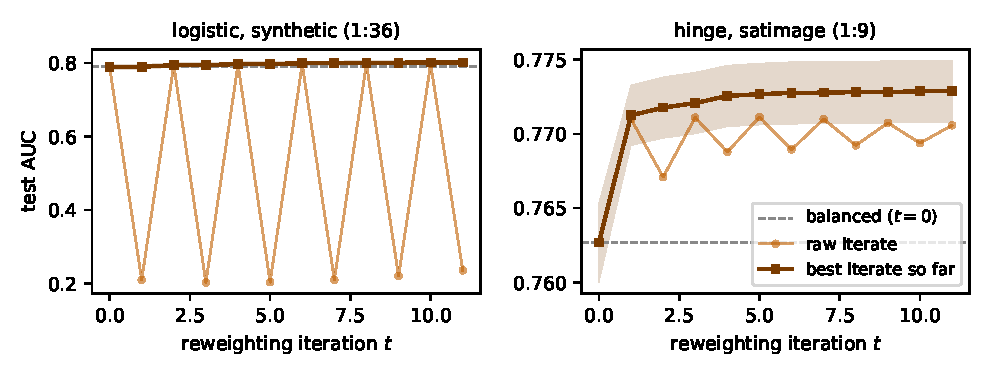
\includegraphics[width=0.92\textwidth]{Figures/auc_vs_iteration.pdf}
\caption{Test AUC by reweighting round (mean $\pm$ standard error over 15
folds, fixed $C = 1$; grey dashed line: balanced fit, $t = 0$). Thin
curve: raw iterates. On the extreme-imbalance synthetic set (left,
logistic base learner) the raw sequence \emph{oscillates}: a full refit at
the new counts is a jump to a polytope vertex with no line search, weight
mass concentrates on the few violated examples, and successive vertices
over-correct, alternating between strong and inverted rankings. Bold
curve: best-iterate-so-far per fold, the quantity harvested by
cross-fitted selection ($+0.6$ points over balanced on the left; right:
hinge base learner on satimage). Near-balanced datasets are flat at the
dashed line (not shown).}
\label{fig:auc_iter}
\end{figure}

\paragraph{1. Count reweighting reproduces pairwise training.} A linear SVM
wrapped in Algorithm~\ref{alg:fwbpr} (margin 2) matches an explicit RankSVM
(pairwise hinge on difference vectors) on all seven datasets: mean paired
AUC differences are at most $0.004$ and per-fold wins split evenly. The same
holds for MLPs: per-epoch count-refreshed weighted cross-entropy tracks full
pairwise-logistic training within noise on all four datasets tried (winning
$5/5$ and $4/5$ paired splits on two of them), while a pairwise epoch costs
$1.3$--$4.4\times$ more at these sizes and scales as $O(n^+ n^-)$ against
$O(N \log N)$. The gradient identity itself was verified through an MLP by
automatic differentiation: hinge gradients agree \emph{exactly} (difference
$0$ in float64), logistic gradients to $10^{-13}$.

\paragraph{2. Iterating is a free option over balancing.} With cross-fitted
joint selection of $(C, t)$, FW-BPR-logistic gains $+0.6$ AUC points over
balanced logistic on the dataset with headroom (synthetic $1{:}36$, winning
$10/15$ folds, median selected $t = 6$) and \emph{selects $t = 0$} -- i.e.,
returns the balanced solution, at no loss -- where balancing is already
optimal (Figure~\ref{fig:auc_iter}). Selection over iterates is not
optional: the raw refit sequence is vertex-hopping without line search and
can oscillate on extreme imbalance (Figure~\ref{fig:auc_iter}, left) --
the discrete analogue of Frank--Wolfe's need for step sizes or convex
combinations \citep{jaggi2013}. Under naive single-split selection the
harvestable gains are destroyed by selection noise; the small validation
sets of heavily imbalanced problems contain few positives, and this, not
the optimization, is the binding constraint.

\paragraph{3. The negative results are the theory's own predictions.}
Balanced logistic regression already matches RankSVM everywhere (winning up
to $14/15$ folds on some datasets) -- the first Frank--Wolfe step plus
AUC-consistency \citep{kotlowski2011,agarwal2014} predicts precisely this
-- and neither pairwise training nor its count-reweighted equivalent
broadly beats plain or balanced cross-entropy on generic tabular data. Any
contrary claim would contradict the consistency of the univariate
baselines. The practical role of the equivalence is therefore cost
reduction and certification wherever pairwise objectives are genuinely the
right tool (ranking heads, verification, deep AUC maximization
\citep{yuan2021}), not headline accuracy.

\paragraph{4. Interpolating learners collapse, as predicted.} Wrapping
gradient-boosted trees drives training AUC to $1.0$, all hard counts to
zero, and Algorithm~\ref{alg:fwbpr} provably returns the balanced fit
(identical AUC to four decimals); static balancing itself does not help
boosting on these datasets. Rescuing interpolating learners requires
out-of-fold count estimation or calibrated margins, which we leave open.

\section{Discussion}
\label{sec:discussion}

The pairwise hinge for bipartite ranking and balanced cost-sensitive
classification are one optimization problem seen from two coordinate
systems, glued by a transportation polytope. The efficiency tricks of
\citet{joachims2005} and \citet{chapelle2010}, the lambdas of
LambdaMART, and the hardness weights of example-mining heuristics are all
shadows of the same object; the polytope adds what the tricks lack -- an
exact domain, a membership certificate, and a sandwich bound on the
remaining gap. The equivalence also delimits its own practical value: since
balanced univariate training is the first step of the pairwise optimization
and is already AUC-consistent, no method in this family can dominate strong
univariate baselines at scale, and our experiments bear this out. Where
pairwise objectives earn their cost -- verification, metric-learning
decision layers, extreme-imbalance regimes with limited positives
\citep{yang2022} -- the identity of
Proposition~\ref{prop:gradient} replaces them at univariate cost, and the
certificate says how far from pairwise-optimal any reweighted solution
sits. Extending the count refresh to interpolating learners via
cross-fitting, and testing the substitution inside deep AUC-maximization
pipelines, are the natural next steps.

\bibliographystyle{plainnat}
\bibliography{references}

\end{document}
